\chapter{Introduzione}\label{introduzione}

La laringoscopia è una procedura medica utilizzata per ispezionare la laringe e per diagnosticare, ed eventualmente curare, i disturbi della laringe e delle corde vocali.

In particolare ci sono due tipi di laringoscopia, quella indiretta e quella diretta. La prima fa uso di un semplice specchio e di una fonte luminosa, la seconda richiede l'uso di un laringoscopio e una anestesia.

Il laringoscopio è uno strumento che grazie a una fibra ottica, una sorgente luminosa e una telecamera permette di osservare nei minimi dettagli la laringe e tutti gli elementi che la costituiscono come la epiglottide e le corde vocali \cite{giorgio_cenni_2008}. In particolare permette di aiutare a diagnosticare malattie come la laryngeal squamous cell carcinoma (SCC), la cui diagnosi precoce riduce la mortalità del paziente \cite{moccia_larynge}.

\begin{figure}[ht]
    \centering
    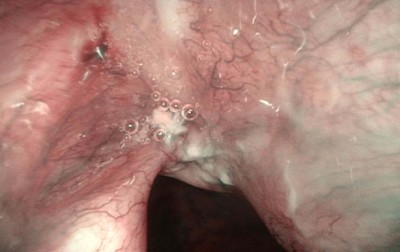
\includegraphics[width=0.3\textwidth]{introduzione/Larynge-1.jpg}
    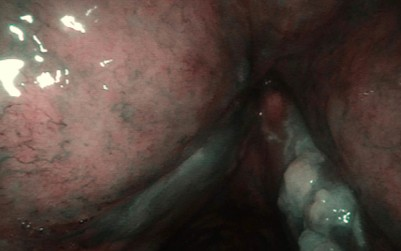
\includegraphics[width=0.3\textwidth]{introduzione/Larynge-2.jpg}

    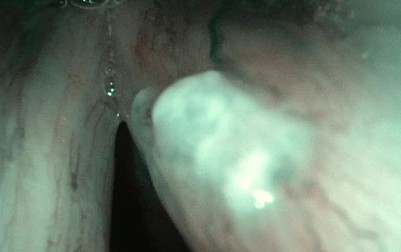
\includegraphics[width=0.3\textwidth]
    {introduzione/Larynge-3.jpg}
    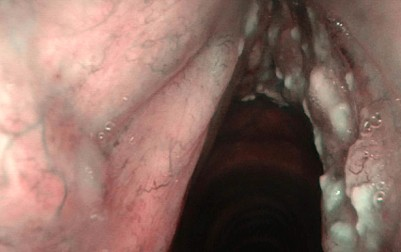
\includegraphics[width=0.3\textwidth]{introduzione/Larynge-4.jpg}
    \caption{Esempio di fotogrammi endoscopici laringei}
    \label{fig:larynges}
\end{figure}

L'obiettivo di questa tesi è quello di usare algoritmi di apprendimento automatico basati sul transfer learning per la classificazione dei frame di una laringoscopia, il  preprocessing di immagini e il data augmentation per ottimizzare l'addestramento. In particolare ci concentriamo nella selezione degli informative-frame e lo scarto di tutti i frame non utili: come frame pieni di saliva o non a fuoco. In \cref{fig:larynges} alcuni esempi di frame da selezionare estratti da una laringoscopia.

\section{Descrizione dei dataset}\label{descrizione-dei-dataset}

L'addestramento della rete è stato effettuato  sul dataset
NBI-InfFrames. Il dataset
è stato realizzato a partire dai frame di 18 video endoscopici NBI, presi dalle laringoscopie di
18 diversi pazienti affetti da carcinoma a cellule squamose
(SCC). Tutti i video sono stati acquisiti con un sistema endoscopico
NBI (processore video Olympus Visera Elite S190 e
un videoscopio rino-laringo ENF-VH) con frame rate di
25 fps e dimensioni dell'immagine di \(1920\times 1072\times 3\) pixel.

\begin{figure}[ht]
    \centering
    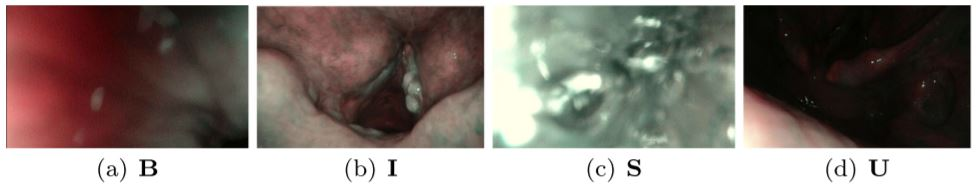
\includegraphics[width=0.9\textwidth]{introduzione/Larynge.jpg}
    \caption[Esempio di fotogrammi endoscopici laringei di NBI-InfFrames]{Esempio di fotogrammi endoscopici laringei di NBI-InfFrames divisi per I: informative, sfuocato: B, S: con
    saliva o riflessi speculari,
    U: underexposed}
    \label{fig:larynges-2}
\end{figure}

Il dataset NBI-InfFrames contiene 720 frame, che sono equamente divisi in quattro classi: informative (I), sfuocato (B), con saliva o riflessi speculari (S) e underexposed  (U), come mostrato in \cref{fig:larynges-2}. 

Dato il basso numero di immagini, il fatto che il dataset sia diviso in maniera omogenea tra le 4 classi fa sì che il modello di apprendimento si focalizzi su tutte le classi e non solo sulla classe predominante, come per esempio gli informative-frame, e ignorando le classi poco diffuse.

Quando c'è eterogeneità tra il numero di pattern per classi il modello di addestramento non riesce ad ottenere risultati ottimizzati in quanto l'algoritmo non tiene conto delle classi poco numerose. Nel caso in cui il modello non riesca a trovare un modello di separazione tra le classi c'è il rischio di overfitting nelle classi con meno dati in quanto impara tutte le feature a memoria. Inoltre è difficile trovare altri dati per convalidare ed effettuare dei test \cite{chatterjee_deep_2018}.

Per ciascuno dei 18 video endoscopici NBI, i fotogrammi video sono stati estratti a caso e
presentati prima a due valutatori umani. Poi, ai due valutatori è stato chiesto di etichettare i fotogrammi. Nel caso in cui i due
valutatori non fossero d'accordo sulla classe, a un terzo valutatore è stato
chiesto di scegliere la classe definitiva tra le due proposte
dai due valutatori. Questo processo è stato ripetuto fino a quando sono stati estratti e classificati dai video 720 fotogrammi divisi in 4 classi equidimensionale \cite{moccia_larynge}.

Il secondo dataset è basato sugli informative-frame del dataset precedente, in particolare è stato effettuato un ritaglio delle immagini per mostrare   alcuni dettagli del tessuto umano, il procedimento è mostrato nella \cref{fig:dataset2}. In \cref{fig:dataset2ml} sono mostrati alcuni frame catalogati il dataset 2 è catalogato in base allo stato del tessuto, in particolare Blu: tessuto con intraepithelial papillary capillary loop-like vessels; Giallo: tessuto con Leukoplakia;
Verde: tessuto sano; Rosso: tessuto con hypertrophic vessels \cite{moccia_larynge}.

Il secondo dataset è composto da 330 immagini, e la dimensione è simile a dataset utilizzati in ricerche sullo stato di salute delle laringi come in \cite{narbalata_larynge} \cite{turkmen_larynge} di rispettivamente 120 e 70 immagini.

\begin{figure}[ht]
    \centering
    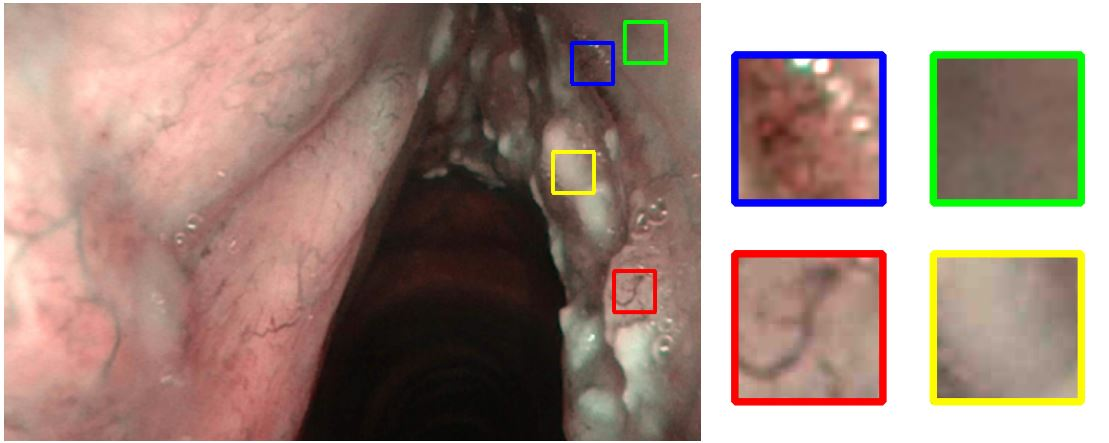
\includegraphics[width=0.9\textwidth]{introduzione/dataset-2.JPG}
    \caption{Esempio di come sono state estratte le immagini del dataset 2}
    \label{fig:dataset2}
\end{figure}

\begin{figure}[ht]
    \centering
    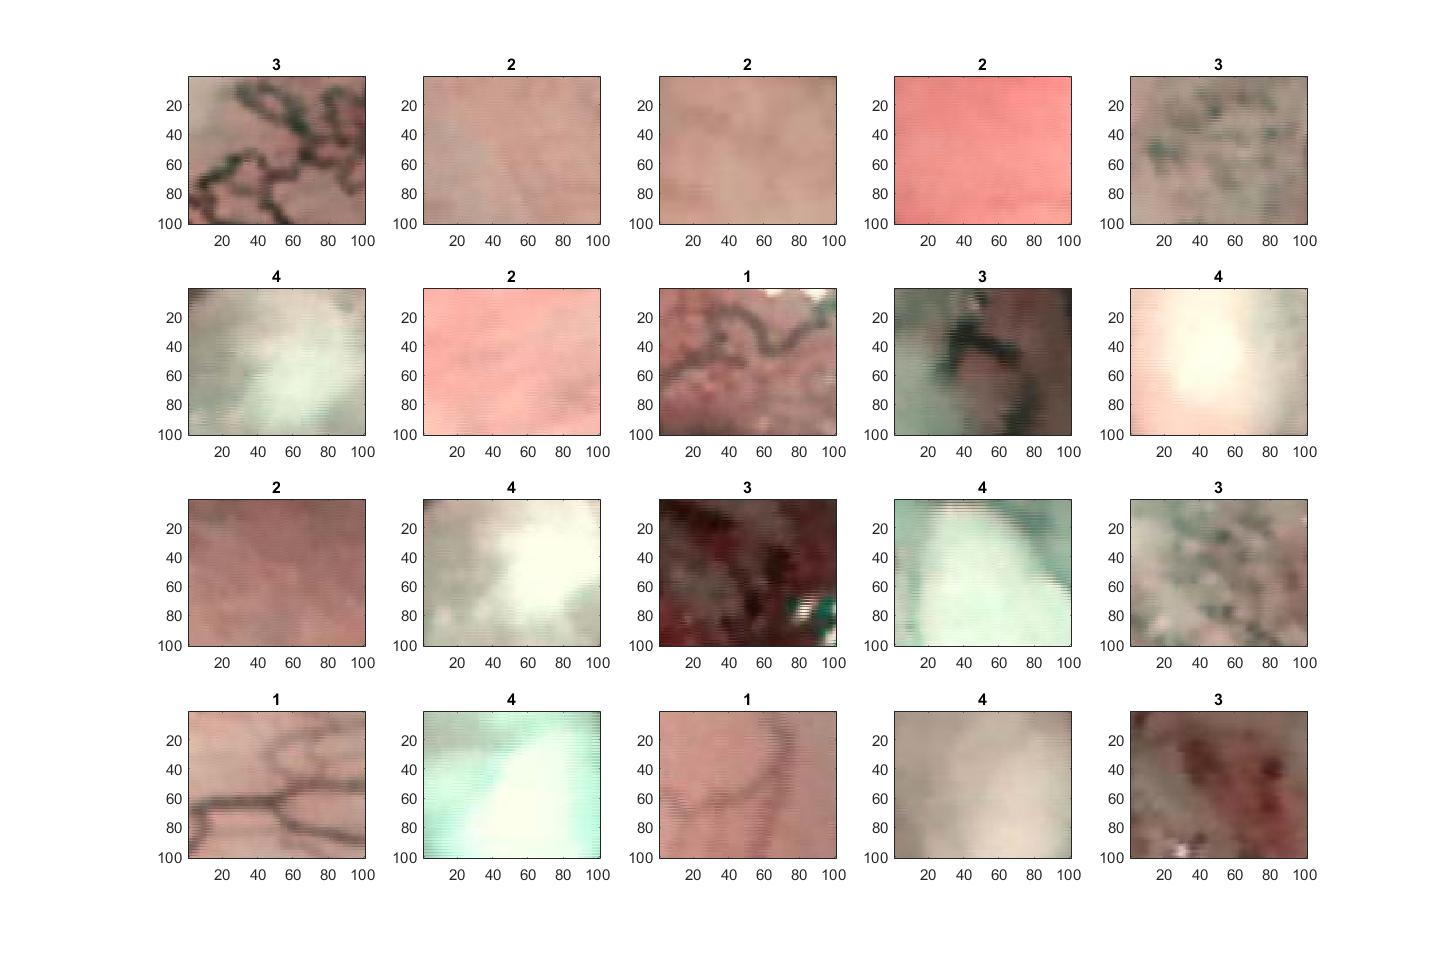
\includegraphics[width=0.9\textwidth]{introduzione/dataset-2-ml.JPG}
    \caption[Esempio di immagini del dataset 2]{Esempio di immagini del dataset 2, le varie classi sono suddivise in base allo stato del tessuto in relazione alla SCC.}
    \label{fig:dataset2ml}
\end{figure}

\section{Lavori precedenti}\label{lavori-precedenti}

Il problema  della classificazione delle immagini e della selezione degli informative-frame è molto presente nel panorama scientifico. L'ImageNet Large Scale Visual Recognition Challenge (ILSVRC) valuta le performance dei vari algoritmi di intelligenza artificiale su una vasta scala, ma non sulla selezione degli informative frame \cite{imagenet}. Le varie soluzioni hanno permesso di ottenere performance sempre superiori, soprattutto a partire dall'introduzione delle reti profonde, che possono essere utilizzate anche per la selezione degli informative-frame.

Per implementare algoritmi in grado di identificare e scartare le immagini non informative nei video endoscopici, sono stati proposti diversi approcci di apprendimento automatico (ML), che sono principalmente basati su handcrafted features, come features basate sull'intensity e sui colori, in \citeauthor{zhang_colon} \cite{zhang_colon} sono state utilizzate caratteristiche anatomiche per la classificazione degli informative frame, mentre caratteristiche sullo stato dell'immagine come colori, sfuocatura, sono stati usati in \citeauthor{armin_colonscopy} \cite{armin_colonscopy}. 

Caratteristiche basate sulla rappresentazione spettrale sono trattate invece in \citeauthor{atasoy_endoscopic} \cite{atasoy_endoscopic}, \citeauthor{haji_wce} \cite{haji_wce} e in \citeauthor{bashar_endoscopy} \cite{bashar_endoscopy} caratteristiche dei colori dell'immagine, come l'istogramma. Nell'ambito della selezione di informative-frame nelle laringi troviamo alcune applicazioni in \citeauthor{moccia_workflow} \cite{moccia_workflow} \citeauthor{moccia_larynge_2} \cite{moccia_larynge_2} e \citeauthor{patrini_tl} \cite{patrini_tl}. La selezione degli informative-frame è molto utile per lavori di selezione per diagnosi precoci di malattie laringee, troviamo alcune applicazioni in \citeauthor{moccia_larynge} \cite{moccia_larynge} \citeauthor{turkmen_larynge} \cite{turkmen_larynge} e \citeauthor{narbalata_larynge} \cite{narbalata_larynge}.

Questa tesi è organizzata come segue: il \cref{transfer-learning} presenta l'approccio di transfer learning utilizzato per selezionare gli informative frame, \cref{frame} spiega come funziona l'acquisizione e la rappresentazione dell'immagine in digitale, \cref{data-augmentation}  e  \cref{preprocessing} spiegano i principali metodi utilizzati per migliorare le performance. I risultati sono mostrati in \cref{addestramento-rete-neurale} e sono discussi nel \cref{conclusioni}.